\documentclass[
ngerman,
twoside,
pdfa=false,
ruledheaders=section,%Ebene bis zu der die Überschriften mit Linien abgetrennt werden, vgl. DEMO-TUDaPub
class=report,% Basisdokumentenklasse. Wählt die Korrespondierende KOMA-Script Klasse
thesis={type=sta},% Dokumententyp Thesis, für Dissertationen siehe die Demo-Datei DEMO-TUDaPhd
accentcolor=TUDa-2c,% Auswahl der Akzentfarbe
custommargins=false,% Ränder werden mithilfe von typearea automatisch berechnet
marginpar=false,% Kopfzeile und Fußzeile erstrecken sich nicht über die Randnotizspalte
%BCOR=5mm,%Bindekorrektur, falls notwendig
parskip=half-,%Absatzkennzeichnung durch Abstand vgl. KOMA-Sript
fontsize=11pt,%Basisschriftgröße laut Corporate Design ist mit 9pt häufig zu klein
%	logofile=tuda_logo.pdf, %Falls die Logo Dateien nicht installiert sind
]{tudapub}

%%%%%%%%%%%%%%%%%%%%%%%%%%%%
% Download des TU-Logos
%%%%%%%%%%%%%%%%%%%%%%%%%%%%
% https://download.hrz.tu-darmstadt.de/protected/CE/TUDa_LaTeX/tuda_logo.pdf
% Der Pfad zum Logo kann als "logofile" angegeben werden.

%%%%%%%%%%%%%%%%%%%
% Sprachanpassung & Verbesserte Trennregeln
%%%%%%%%%%%%%%%%%%%
\usepackage[english, main=ngerman]{babel}
\usepackage[autostyle]{csquotes}% Anführungszeichen vereinfacht
\usepackage{microtype}

%%%%%%%%%%%%%%%%%%%
% Literaturverzeichnis
%%%%%%%%%%%%%%%%%%%
\usepackage{biblatex}   % Literaturverzeichnis
\addbibresource{HausarbeitBib.bib}

%%%%%%%%%%%%%%%%%%%
% Paketvorschläge Tabellen
%%%%%%%%%%%%%%%%%%%
%\usepackage{array}     % Basispaket für Tabellenkonfiguration, wird von den folgenden automatisch geladen
\usepackage{tabularx}   % Tabellen, die sich automatisch der Breite anpassen
%\usepackage{longtable} % Mehrseitige Tabellen
%\usepackage{xltabular} % Mehrseitige Tabellen mit anpassarer Breite
\usepackage{booktabs}   % Verbesserte Möglichkeiten für Tabellenlayout über horizontale Linien

%%%%%%%%%%%%%%%%%%%
% Paketvorschläge Mathematik
%%%%%%%%%%%%%%%%%%%
\usepackage{mathtools} % erweiterte Fassung von amsmath
\usepackage{amssymb}   % erweiterter Zeichensatz
\usepackage[decimalsymbol=comma]{siunitx}   % Einheiten
\usepackage{amsmath}


%%%%%%%%%%%%%%%%%
% Eigenen Pakete Gruppe01
%%%%%%%%%%%%%%%%%%%%
%\usepackage[utf8]{inputenc}
%\usepackage[ngerman]{babel}
\usepackage{hyperref}
\usepackage{graphicx}
\usepackage{subcaption}
\usepackage{listings}
\usepackage[framed, numbered]{matlab-prettifier}
%\usepackage[style=numeric]{biblatex}
%\usepackage{amsthm}
%\usepackage[squaren]{SIunits}
\usepackage{enumitem}
\usepackage{tikz}
\usepackage{pgfplots}
\usepackage{pgfplotstable}
%\usepackage{booktabs}
\pgfplotsset{compat=1.12}
\usepackage{dsfont}
\usepackage{arcs}

\usepackage{media9}

%%%%%%%%%%%%%%%%%%%
% verschiedene Nummerierung für Abbildungen und Formeln
%%%%%%%%%%%%%%%%%%%
\usepackage{chngcntr}
%\counterwithout{equation}{chapter}


%%%%%%%%%%%%%%%%%%%
% Pseudocode
%%%%%%%%%%%%%%%%%%%
\usepackage[linesnumbered,lined,boxruled]{algorithm2e} % Package für Pseudocode

%%%%%%%%%%%%%%%%%%%
% Plotting und Grafik
%%%%%%%%%%%%%%%%%%%
\usepackage{tuda-pgfplots} % Package für Plotting with TUDa mods

%%%%%%%%%%%%%%%%%%%
% Sonstiges
%%%%%%%%%%%%%%%%%%%
\usepackage{blindtext} % Package für Blindtext

\renewcommand{\tt}[1]{\texttt{#1}} 
\newcommand{\m}[1]{\textrm{#1}} 
\renewcommand{\b}[1]{\textbf{#1}} 
\newcommand{\mb}[1]{\mathbf{#1}} 


\begin{document}
	
	\title{Ausarbeitung Übung 9}
	%\subtitle{Ein Untertitel, wenn nötig}
	\author[D. Schiller, C. Kramer, S.Arnold, T. Lingenberg]{Dominik Schiller \and Constanze Kramer \and Simon Arnold \and Tobias Lingenberg} %optionales Argument ist die Signatur,
	%\reviewer{Gutachter 1 \and Gutachterin 2} %Gutachten
	
	%Diese Felder werden untereinander auf der Titelseite platziert.
	\department{} % Das Kürzel wird automatisch ersetzt und als Studienfach gewählt, siehe Liste der Kürzel im Dokument.

	
	\date{\today}
	%\examdate{\today}
	
	%	\tuprints{urn=1234,printid=12345}
	%	\dedication{Für alle, die \TeX{} nutzen.}
	
	\maketitle
	\pagenumbering{gobble} % Seitenzahlen angezeigt, startet ab dem Inhaltsverzeichnis
	
	
	%\affidavit
	%\AffidavitSignature
	%\AffidavitSignature
	
	
	%%%%%%%%%%%%%%%%%%%
	%Abstract / Kurzzusammenfassung
	%%%%%%%%%%%%%%%%%%%
	%\include{chapters/zusammenfassung}
	
	%%%%%%%%%%%%%%%%%%%
	%Inhaltsverzeichnis 
	%%%%%%%%%%%%%%%%%%%
	\cleardoublepage
	\tableofcontents % Erstellte ein Inhaltsverzeichnis
	
	%\cleardoublepage
	\pagenumbering{arabic} % Seitenzahlen angezeigt, startet ab dem Inhaltsverzeichnis
	\setcounter{page}{1} % Setzt den Seitenzahlenzähler auf 1
	
	%%%%%%%%%%%%%%%%%%%%%%%%%%%%%%%%%%%%%%%%%%%%%%%%%%%%%%%%%%%%%%%%%%%%%%%%%%%%%%%%%%%%%%%%%%%%%%%%%%
	
	% INHALT, am Besten ausgelagert in eigene Files/Kapitel und dann mit \include{Unterordner/Filename} eingefügt, sorgt für bessere Übersichtlichkeit und Fehlersuche. Einzelne Dateien sind aktuell im Ordner Sections abgelegt. 
	%%%%%%%%%%%%%%%%%%Einleitung%%%%%%%%%%%%%%%%%
	\chapter{Einleitung}\label{sec:intro}
Diese Arbeit beschäftigt sich mit dem Übungsblatt 9 des Faches \glqq Einführung in die numerische Berechnung elektromagnetischer Felder\grqq{}.
Zunächst wird der primale Divergenz und Rotationsoperator in Octave implementiert und berechnet. Anschließend wird eine Materialmatrix berechnet. Abschließend wird das Magnetfeld von zwei stromdruchflossenen Leitern in Octave simuliert. 
	%%%%%%%%%%%%%%%%%%Haupteil%%%%%%%%%%%%%%%%%%%
	\chapter{Ausarbeitung der Aufgaben}
\section{Rotationsoperator}
Zur numerischen Berechnung der allgemeinen Vektordifferentialgleichung der Magnetostatik $$ \m{rot}\left( \mu^-1(\vec{r})\m{rot}\vec{A}(\vec{r})\right) = \vec{J}(\vec{r}) $$ wird der Rotationsoperator benötigt. Dieser lässt sich, wie schon der Divergenzoperator, mit dem diskretisierten partiellen Ableitungsoperator
\begin{equation} 
(\mb{P}_w)_{p,q} := \delta_{p+M_w,q} - \delta{p,q} =  
\begin{cases} 
-1 & \m{für    }  q = p \\ 
+1 & \m{für    }  q = p + M_w \\ 
0 & \m{sonst}	 
\end{cases}, \m{wobei } w = x,y,z 
\label{eq:Ableitung} 
\end{equation}  bestimmen. Es lassen sich nun unterschiedliche Operatoren erzeugen, zunächst der Rotationsoperator 
\begin{equation*}
	\mb{C} = 
	\begin{bmatrix}
	\mb{0} & -\mb{P}_z & \mb{P}_y \\
	\mb{P}_z & \mb{0} & -\mb{P}_x \\
	-\mb{P}_y & \mb{P}_x & \mb{0}
	\end{bmatrix},
\end{equation*} der diskrete div-Operator auf dem primalen Gitter 
\begin{equation*}
	\mb{S} = \begin{bmatrix}
	\mb{P}_x & \mb{P}_y & \mb{P}_z
	\end{bmatrix},
\end{equation*} sowie der duale Divergenzoperator
\begin{equation*}
\tilde{\mb{S}} = \begin{bmatrix}
-\mb{P}_x^T & -\mb{P}_y^T & -\mb{P}_z^T
\end{bmatrix}.
\end{equation*}\\ \\
Die angehängte Methode \tt{fit\_operator} berechnet diese Operatoren auf einem der Methode übergebenen Gebiet und liefert sie zurück. \\
Allgemein gilt $\nabla\cdot(\nabla\times\vec{A}) = 0$, diese Identität lässt sich auch mit den primalen Rotations- und Divergenzoperator nachprüfen. Multipliziert man den Divergenzoperator \b{S} auf den Rotationsoperator ergibt sich
\begin{equation}
	\begin{split}
		\mb{SC} &= \begin{bmatrix}
		\mb{P}_x & \mb{P}_y & \mb{P}_z
		\end{bmatrix} \cdot
		\begin{bmatrix}
		\mb{0} & -\mb{P}_z & \mb{P}_y \\
		\mb{P}_z & \mb{0} & -\mb{P}_x \\
		-\mb{P}_y & \mb{P}_x & \mb{0}
		\end{bmatrix}\\\\
		&= \begin{bmatrix}
		\mb{P}_y\mb{P}_z-\mb{P}_z\mb{P}_y & & -\mb{P}_x\mb{P}_z+\mb{P}_z\mb{P}_x & & \mb{P}_x\mb{P}_y-\mb{P}_y\mb{P}_x
	\end{bmatrix}.
	\end{split}
	\label{eq:SC}
\end{equation}
Nutzt man nun die Eigenschaften des Satz von Schwarz und der Kommutativität zweier Matrizen aus, so lässt sich die (\ref{eq:SC}) als 
\begin{equation}
	\mb{SC} = \begin{bmatrix}
	\mb{P}_y\mb{P}_z-\mb{P}_y\mb{P}_z& &-\mb{P}_x\mb{P}_z+\mb{P}_x\mb{P}_z& &\mb{P}_x\mb{P}_y-\mb{P}_x\mb{P}_y
	\end{bmatrix}
\end{equation} schreiben, wodurch sich $$\mb{SC} = \begin{bmatrix}
0 & 0 & 0
\end{bmatrix}$$ ergibt.\\\\
Interpretiert man das Ergebnis geometrisch, wird über jede Fläche eines Volumens integriert. Hierzu wird jede Fläche über Kantenintegrale ausgedrückt. Unter Beachtung der Flächennormalen und der damit verbundenen Integrationsrichtung wird über jede Kante zweimal in unterschiedlicher Richtung integriert. Somit heben sich diese auf, wodurch die ganze Rechnung einen Nullvektor erzeugt.
	\section{Materialmatrix}

Um ein allgemeines magnetostatisches Problem zu lösen benötigt man die Materialmatrix der Reluktivitäten $\textbf{M}_\nu$. Im folgenden werden in jeder Elementarzelle homogene Materialeigenschaften angenommen. Daher lässt sich mit der gemittelten Reluktivität $\bar{\nu}_n$ zwischen zwei benachbarten Zellen, jedes Element $\textbf{M}_\nu (n,n)$ näherungsweise mit 

\begin{equation*}
	\frac{\int_{\tilde{L}_n} \vec{H} \mathrm{d}\vec{s}}{\int_{A_n} \vec{B} \mathrm{d}\vec{A}} \approx \frac{\bar{\nu}_n |\tilde{L}_n|}{|A_n|} =: \textbf{M}_\nu(n,n)
\end{equation*}

bestimmen.
Die dabei entstehende Matrix $\textbf{M}_\nu$ hat Diagonalform.

Die MATLAB Routine \texttt{fit\_calc\_elements} (siehe Code(\ref{kanten})) berechnet die primalen und dualen Flächeninhalte \texttt{dA} und \texttt{ddA} sowie die Kantenlängen \texttt{ds} und \texttt{dds} in Abhängigkeit von den vorgegebenen Gittergrößen \texttt{xmesh, ymesh} und \texttt{zmesh}. Die primalen Kanten entlang einer Achsenrichtung haben alle die selbe Länge \texttt{stepw}, die dualen Kanten berechnen sich je zur Hälfte aus den daneben liegenden primalen Kanten. Daraus folgt das duale Kanten am Rand des Rechengebiets genau halb so lang sind wie die Kanten im Inneren. Die jeweiligen Flächeninhalte ergeben sich aus der Multiplikation der Kantenlänge der angrenzenden Kanten. 

Die Funktion \texttt{fit\_calc\_avgny} (siehe Code (\ref{mittel})) ermittelt den Mittelwert der Reluktiviät zwischen zwei beliebigen, benachbarten Zellen.

Mit Hilfe der zwei schon genannten Funktionen gibt die Funktion \texttt{createMny} (siehe Code(\ref{Matmatrix})) die Materialmatrix $\textbf{M}_\nu$ zurück. Die Einträge sind dabei in $x-$, $y-$ und $z-$Richtung sortiert.

Da am Rand des Rechengebiets zur Mittelung der Reluktivität, zur Hälfte eine nicht vorhandene Zelle mit Reluktivität $\nu = 0$, in die Rechnung einfließt gibt es hier eine kleine Ungenauigkeit und $\bar{\nu}$ ist hier kleiner als es eigentlich sein sollte. 
	\section{Definition eines Stromflusses, Octave}
Wir betrachten nun das Problem zwei parallel verlaufender Kabel (siehe Abb. \ref{fig:problem}). Kabel 1 soll den Strom $1 \si{\ampere}$ und Kabel 2 entgegengesetzt $-1\si{\ampere}$ führen. Angenommen wird, dass die magnetische Flussdichte an den Randflächen $\Gamma$ des Rechengebiets abgeklungen ist und 
\begin{equation}
\label{rand}
\vec{A}_t(\vec{r}) = 0 \qquad \text{für alle } \vec{r} \in \Gamma
\end{equation}
gilt.

\begin{figure}[thbp]
	\centering
	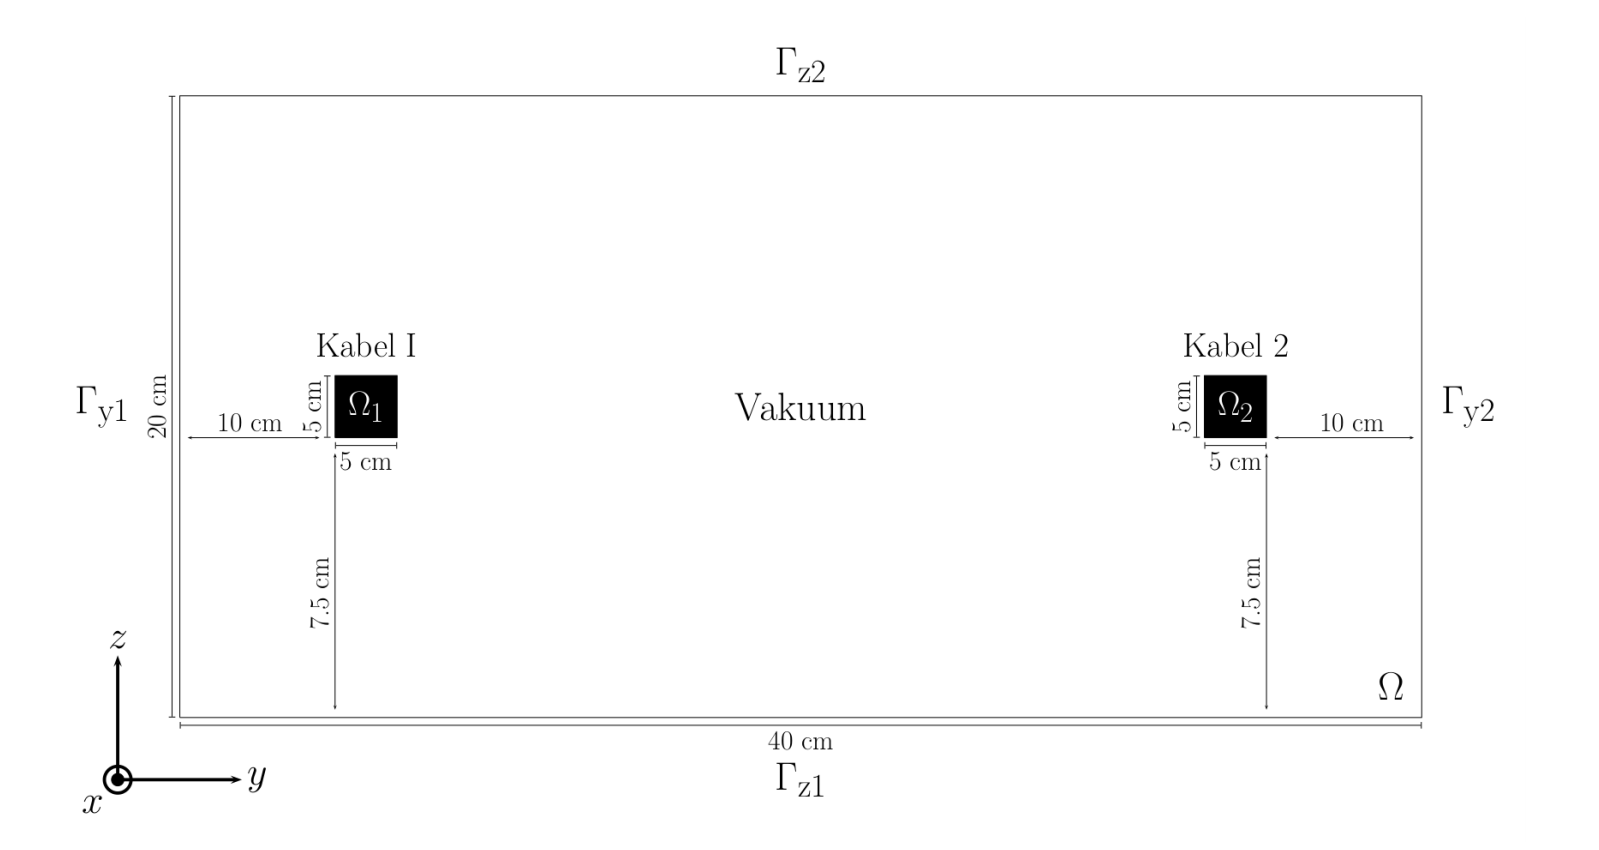
\includegraphics[width=.75\textwidth]{data/Problem}
	\caption{Zwei Kabel in der $yz$-Ebene}
	\label{fig:problem}
\end{figure}

Für die Simulation wird ein äquidistantes Rechengitter definiert. Wir haben uns dazu entschieden zu Testzwecken zunächst einmal ein sehr grobes Gitter zu wählen, mit Anzahl Knoten $N_x=2, N_y=9, N_z=9$ und einer Schrittweite $h_x=20\si{\centi\meter},h_y=5\si{\centi\meter},h_z=2,5\si{\centi\meter}$ (siehe Code (\ref{ag3})). Mithilfe der zuvor geschriebenen Methoden \texttt{fit\_operator} wird der benötigte FIT-Operator $C$ erzeugt. Es folgt die Bestimmung der Indexmenge \texttt{indxT} aller Randkanten, die wir als Vektor definiert haben. Hierbei werden erst alle Kanten in x-Richtung durch gegangen, daran angehängt die in y- und z-Richtung. Im Vektor steht nun entweder eine $1$, falls die Kante eine Randkante ist, ansonsten eine $0$.

Ähnlich wird bei Bestimmung des Anregungsvektors $\vec{j}$ vorgegangen. Der Vektor wird am Index einer Kante, die zum einen in $\Omega_1$ oder $\Omega_2$ liegt und zusätzlich in Stromrichtung (also x-Richtung) zeigt, auf $\pm1$ gesetzt. Anschließend wird der Vektor noch mit dem Faktor $\left(\dfrac{h_x}{5\si{\centi\meter}}\right)^2$ multipliziert.

Nun soll die Gleichung
\begin{equation}
\label{Kaj}
	K\vec{a} = \vec{j} \qquad \text{mit } K = C^TM_vC
\end{equation}
gelöst werden. Hierzu wird zunächst noch mithilfe der schon geschriebenen Routine \texttt{createMny} die Matrix $M_v$ erzeugt. Das magnetische Vektorpotential $\vec{a}$ enthält momentan schon Werte die uns bekannt sind, jene, die durch die Randbedingung (\ref{rand}) festgelegt sind. Es wird eine Zerlegung des Gleichungssystems in Bekannte und Unbekannte vorgenommen. Hierzu werden aus dem Gleichungssystem (\ref{Kaj}) alle Gleichungen entfernt die Randkanten beschreiben. Mithilfe des Vektors \texttt{indxT} werden in $K$ und $\vec{j}$ alle Zeilen (bzw. bei $K$ auch die Spalten) gelöscht, die dem Index einer Randkante entsprechen. Das verkleinerte Gleichungssystem lässt sich nun eindeutig lösen. Die Randbedingung fungiert als eine Form von Eichung.

Zuletzt können nun noch die beiden Gleichungen
\begin{align*}
\vec{b} &= C\vec{a},\\
L &= (\vec{j})^T \dfrac{\vec{a}}{I^2}
\end{align*}
berechnet werden (siehe Code (\ref{ag3}))

Eine Simulation in FEMM ergab das resultierende magnetische Feld (Abb. \ref{fig:magnet}) und den Stromfluss (Abb. \ref{fig:strom}). Der Stromfluss verhält sich nach dem Skineffekt so wie erwartet (Am Rand des Kabels ist ein erhöhter Stromfluss erkennbar). Wieder den Erwartungen verhält sich jedoch das Magnetfeld (Abb. \ref{fig:magnet}) durch Bedingung (\ref{rand}) sollte es am Rand des Rechengebiets $0$ sein.

\begin{figure}[thbp]
	\centering
	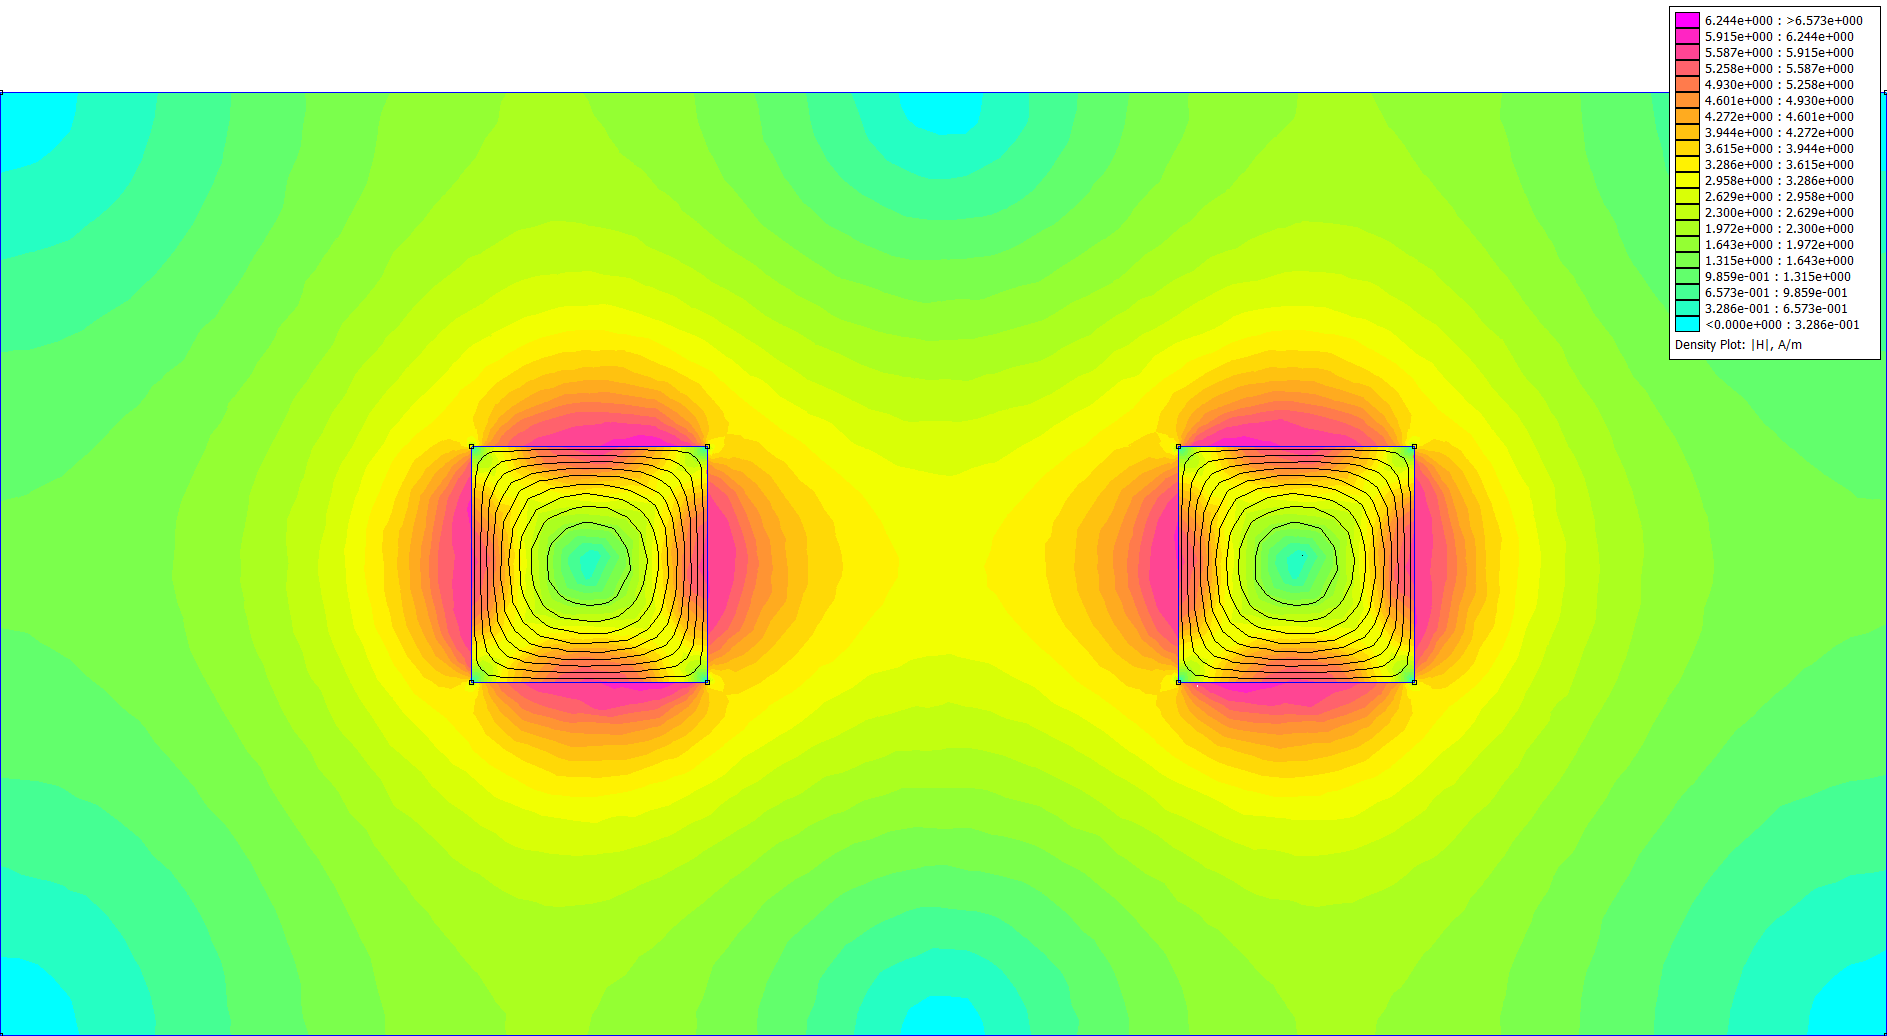
\includegraphics[width=.68\textwidth]{data/MagnetischesFeld}
	\caption{Simulation des Magnetischen Feldes in FEMM}
	\label{fig:magnet}
\end{figure}

\begin{figure}[thbp]
	\centering
	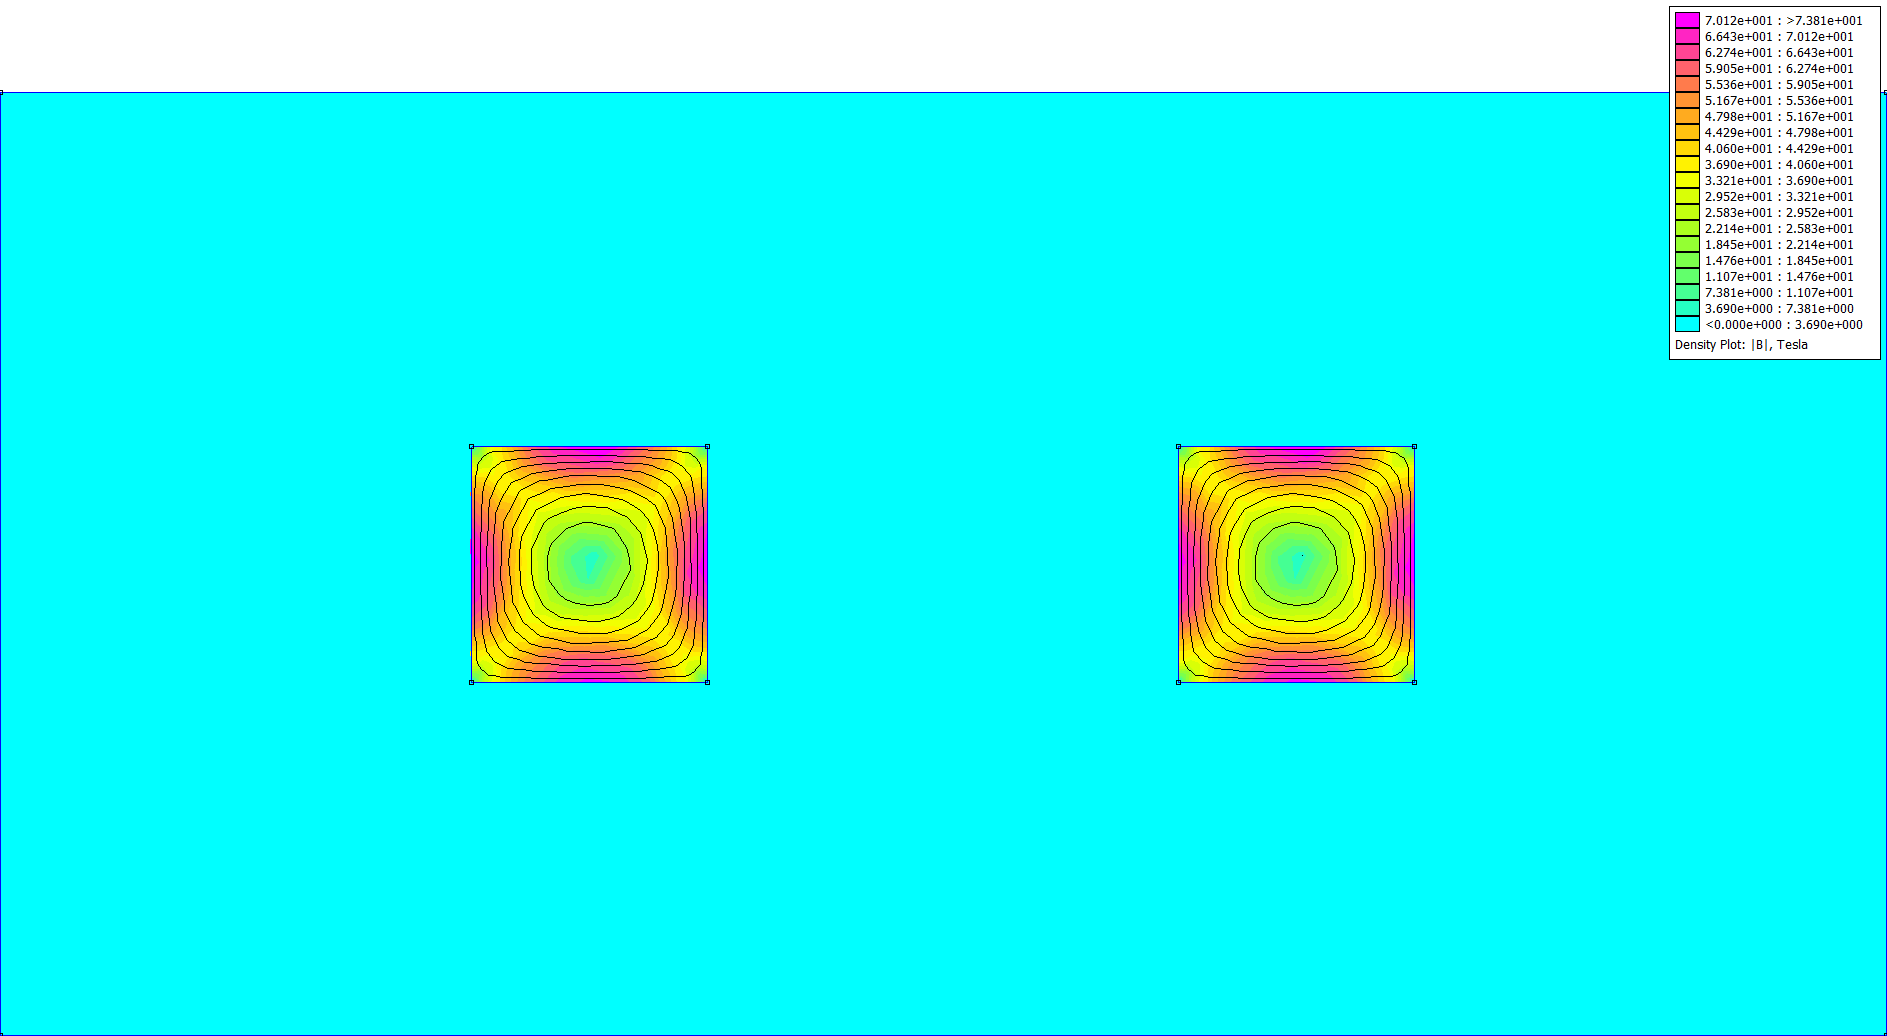
\includegraphics[width=.68\textwidth]{data/Stromfluss}
	\caption{Simulation des Stromflusses in FEMM}
	\label{fig:strom}
\end{figure}
	%%%%%%%%%%%%%%%%%%Fazit%%%%%%%%%%%%%%%%%%%%%%
	\chapter{Fazit}\label{sec:fazit}
%\addcontentsline{toc}{section}{Fazit}
Die erste Aufgabe ergab, dass sich die beiden Leiter des Koaxialkabels wie die Platten eines Plattenkondensators verhalten. Darüber hinaus ergibt sich, dass man durch Anfügen von weiteren Segmenten an die Schaltung eine Verkleinerung der Schwingfrequenz bewirkt.
Differentialgleichungen können häufig, wie sich in Aufgabe zwei zeigt, leichter im Frequenzbereich als im Zeitbereich gelöst werden. Die durch Lösen der Differentialgleichung analytisch berechneten Ergebnisse für Zeit- und Frequenzverhalten stimmen dabei mit der numerischen Simulation durch LTSpice überein.
Die Ergebnisse der dritten Aufgabe ergeben, dass sich die Feldlinien eines Kondensators in einem Simulationskäfig nicht nur senkrecht zu den Platten bewegen, sondern dass sich auch Randeffekte an den Enden der Kondensatorplatten ausbilden. Untersucht man unterschiedliche Randbedingungen zeigt sich, dass diese sowohl den Kapazitätswert des Kondensators, als auch die elektrischen Feldlinien beeinträchtigen. Die Wahl der Simulationsrandbedingungen kann also nicht willkürlich erfolgen.
	%%%%%%%%%%%%%%%%%%Anhang%%%%%%%%%%%%%%%%%%%%%
	\chapter{Anhang}\label{sec:anhang}
\lstset{ % Octave Settings
	language=Octave,
	extendedchars=true,
	basicstyle=\footnotesize,
	numbers=left,
	numberstyle=\tiny\color{gray},
	stepnumber=1,
	numbersep=10pt,
	showspaces=false,
	showstringspaces=false,
	tabsize=2,
	breaklines=true,
	frame=single,
	morecomment = [l][\itshape\color{blue}]{\%},
	captionpos=b,
	title=\lstname
}


\lstinputlisting{data/SIS.m}
\lstinputlisting{data/SkriptAg8_2.m}
\lstinputlisting{data/SkriptAg8_3d.m}



	%%%%%%%%%%%%%%%%%%%%%%%%%%%%%%%%%%%%%%%%%%%%%%%%%%%%%%%%%%%%%%%%%%%%%%%%%%%%%%%%%%%%%%%%%%%%%%%%%%
	
	%%%%%%%%%%%%%%%%%%%
	%Abbildungs- und Tabellenverzeichnis
	%%%%%%%%%%%%%%%%%%%
	\listoffigures % Abbildungsverzeichnis (captions in den Figuren werden als Referenz genommen)
	%\listoftables % Verzeichnis der Tabellen (captions in den Tabellen werden als Referenz genommen)
	
	%%%%%%%%%%%%%%%%%%%
	%Literaturverzeichnis an dieser Stelle
	%%%%%%%%%%%%%%%%%%%
	
	
\end{document}
